\chapter{System Validation}\label{ch:validation}

\textcolor{red}{THIS IS AN UNFINISHED CHAPTER}

This chapter presents the validation of the proposed solution.
The validation process is described into different sections, each addressing different components of the system.
Section~\ref{sec:meth} outlines the methodology used for validation.
Section~\ref{sec:core_network} describes the Core network setup.
Section~\ref{sec:flexric} details the FlexRIC solution used in the system.
Section~\ref{sec:gnb} details the gNB configuration and validation.
Section~\ref{sec:ue} addresses the User Equipment (UE) setup and tests.
Section~\ref{sec:cv_module} discusses the computer vision module and its integration.
Section~\ref{sec:mm_xapp} focuses on the Mobility Management xApp and its role in the system .
Section~\ref{sec:use_case} presents a specific use case to demonstrate the system's functionality.
Finally, Section~\ref{sec:discuss} provides a discussion of the results and insights gained from the validation process.

\section{Methodology}\label{sec:meth}
This section describes the overall methodology employed to validate the system.
It includes details on the experimental setup, data collection methods, and the criteria used for evaluation.

\section{Core Network}\label{sec:core_network}
In this section, the core network configuration and validation are discussed.
It includes the setup of network elements, their interactions, and performance metrics.
In order to make sure that all Core Network components are working properly, we performed a test.
The deployment of the Core Network is done through Docker containers.
Figure~\ref{fig:core_init} presents the command for running the Core Network setup script.
After the initialization of the Docker containers, it is possible to see the logs of the setup script, indicating the successful initialization.

\begin{figure}[H]
    \centering
    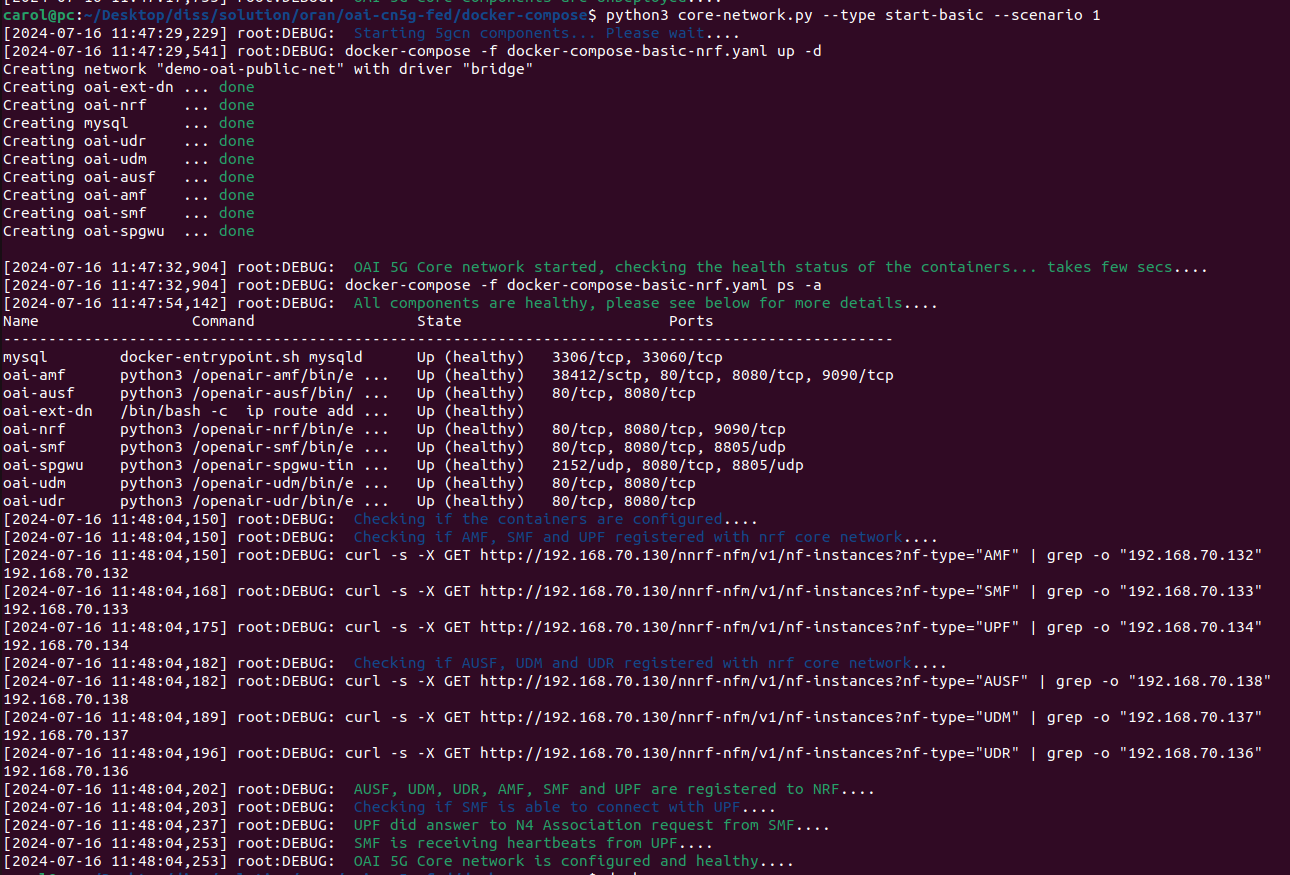
\includegraphics[width=0.5\linewidth]{figures/core_init}
    \caption[Initialization of the Core Network]{Initialization of the Core Network}
    \label{fig:core_init}
\end{figure}

    Then, we verified that all the containers had connectivity using the interface created in the Host OS, using the ping tool,as shown by Figure~\ref{fig:ping_core}.
    Each interface sends requests to each network component according to the table~\ref{}.

\begin{figure}[H]
\centering
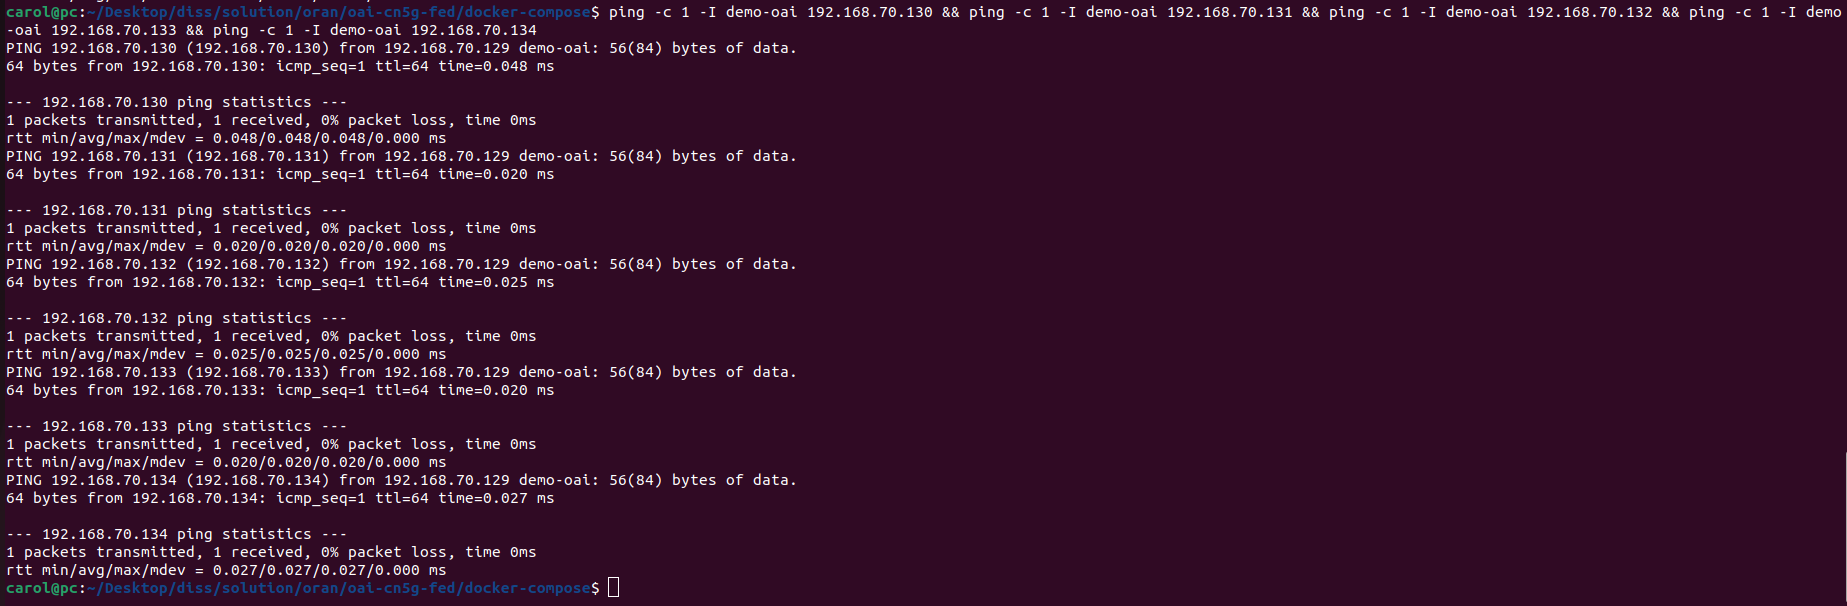
\includegraphics[width=0.5\linewidth]{figures/ping_core}
\caption[Pinging NRF, MySQL Database, AMF, SMF and UPF respectively from Host OS
interface]{Pinging NRF, MySQL Database, AMF, SMF and UPF respectively from Host OS
interface}
\label{fig:ping_core}
\end{figure}

Successfully concluding this tests ensures that the 5G Core Network is operational.



\section{FleXRIC}\label{sec:flexric}
As for the FlexRIC deployment, it is simply necessary to assure its correct launch.
Upon launching, it awaits for incomming connection requests from an E2 Node.
Figure~\ref{} shows the initialization of the FlexRIC.

% launch of FLEXRIC ./nearRT-RIC

\section{gNB}\label{sec:gnb}
To ensure the correct functioning of the gNB, it should be registered in the 5G Core Network, connected to the FlexRIC and registered as a E2 node.
They need to be validated separately since the connections are independent.

To access the gNB connectivity to the Core, we need to check the connection between the gNB Host and the AMF and UPF, since the gNB needs to communicate with them.
This can be tested with ping from the gNB's Host to these entities.
Figure~\ref{} shows the results.

% figure with ping to AMF and UPF 132 and 134

After

\section{UE}\label{sec:ue}
This section discusses the User Equipment (UE) configuration and validation.
It includes the setup of devices, connection procedures, and performance assessments.

\section{Computer Vision Module}\label{sec:cv_module}
The computer vision module is the main developed component in the system of this dissertation, enabling object detection and tracking to enhance dynamic network management.
The computer vision module act as a server to the xApp.
Their interface ensures reliable data exchange using a socket connection, leveraging an ASN.1 file to standardize the structure of the messages.

To ensure the correctness and reliability of the computer vision module, a series of validation tests were conducted.
These tests were designed to evaluate both the processing capabilities of the module and the accuracy of the message exchange between the vision module and the xApp.

The processing time of each frame was measured to assess the real-time performance of the computer vision module.
This was critical to ensure that the module could keep up with dynamic environments, such as an office setting where people and objects are constantly moving.
The tests showed that the processing times were within acceptable limits, allowing for timely detection and response.
% show some math on why this result is sufficient
% plot some results

A reference video was used to evaluate the detection and tracking results of the computer vision module.
This video, containing typical office movements like people walking and objects being moved, was processed to check for detection accuracy and tracking consistency.
The results confirmed that the module could accurately detect and track objects, validating its effectiveness in a real-world scenario.

% image of a frame of the video and the corresponding messages

Print statements were used on the server side to verify the correct formatting, coding, and decoding of the messages.
This step was crucial to ensure that the messages sent from the computer vision module to the xApp were correctly structured and could be properly interpreted upon receipt.

On the client side,the xApp, print statements were employed to confirm the correct reception of the messages.
This validation step ensured that the messages transmitted through the socket connection were received intact and could be  correctly processed.

To further validate the communication, Wireshark was used to capture SCTP packets containing the messages exchanged between the server and client.
This capture provided a detailed view of the message flow, confirming that the messages were being transmitted as expected without any loss or corruption.
The capture presents the

% image of the wireshark capture

% MEASURE IF THE SCTP MESSAGES ARE BOTTLENEKING THE APPLICATION.

% maybe define a periodicity for it.


The computer vision module's performance proved adequate for the intended application, i.e.\ an office environment where movements are frequent yet the velocity is low, such as people walking or objects being moved.
The module demonstrated good performance in these scenarios, and its near real-time processing capability can ensure prompt reactions to environmental changes.



\section{Mobility Management xApp}\label{sec:mm_xapp}
This section focuses on the Mobility Management xApp and its role in the system.
It details the design and implementation of the xApp, how it interfaces with other components, and the results of its validation.

\section{Use case}\label{sec:use_case}
In order to validate the implemented solution, a use case testing scenario was established.
In an indoor environment, the system followed the architecture presented in Figure~\ref{fig:}.



The goal of test was to access the functionality of the whole system, considering maintaining end-to-end connection between the UE and the external DN. The Mobile RAN positioning is defined by the mobility management xApp, based on data collected from the Computer Vision Module and the radio metrics collected from the RAN via the Near-RT RIC. It aimed at maintaining the channel quality, or increasing it whenever possible.

The use case shows the system's capabilities in three test scenarios, described in the following subsections.

\subsection{Scenario 0 : Fixed gNB and UE}

In this scenario, the objective is to assess the impact of blockages on the line of sight (LOS) between the gNB (gNodeB) and the UE (User Equipment).
By maintaining a fixed position for both the gNB and the UE, we can introduce obstacles to observe their effects on signal quality and transmission reliability.
This scenario also aims to validate the accuracy of the messages sent by the vision module regarding the presence and nature of these blockages.

The results from this scenario will serve as a baseline for comparison with Scenarios 1 and 2, where the positions of the gNB and UE may vary.
This analysis is important for evaluating the gains of having computer vision solutions integrated into mobile networks.

\subsection{Scenario 1: Moving gNB}
% change it
In this scenario, the User Equipment (UE) encounters an obstacle that obstructs its line of sight. % change specially this sentance
The system promptly identifies the obstacle and predicts when the blockage is expected to happen.
A message indicating the future blockage is sent to the xApp, which then informs the gNB (gNodeB). In response, the gNB preemptively adjusts its position to maintain a clear line of sight with the UE, thereby sustaining a consistent average Signal-to-Noise Ratio (SNR). This proactive approach ensures uninterrupted communication and optimal performance despite the presence of obstacles.

\subsection{Scenario 2: UE Moving Away from the gNB}

This scenario involves the UE moving progressively further from the gNB. In the absence of identified obstacles, a decrease in the Signal-to-Noise Ratio (SNR) is interpreted as the UE increasing its distance from the gNB. To address this, the robotic platform, leveraging the Mobility Management xApp, dynamically moves towards the UE to uphold optimal communication quality.
This adaptive response ensures that the UE remains within the effective communication range of the gNB, thereby maintaining robust and reliable connectivity.


\section{Discussion}\label{sec:discuss}
This section provides a discussion on the results obtained from the validation process.
It includes insights, lessons learned, and potential areas for improvement in future iterations of the system.
